\section{System Demonstration Hardware Setup \label{sec:hardwaresetup}}


(we have more existing materials for this section, to be included soon).

The demonstration system comprises a full trigger path using a single tracking trigger tower (1/48 of the full detector). It uses simulated high-luminosity data as input to measure trigger latency and efficiency, to study overall system performance, and to identify appropriate solutions to possible bottlenecks. 
The demonstration system achieved excellent performance in terms of tracking efficiency and momentum resolution within a very short latency (2.5 microseconds). This latency includes the time needed for data delivery to the trigger towers, for pattern recognition, and for track fitting. This demonstration is proof that fast data delivery, fast pattern recognition, and track fitting can be implemented successfully using the full mesh ATCA architecture and an associative memory approach. While the focus here is on the HL-LHC, the techniques developed are rather generic and could have other applications beyond tracking triggers, within and outside HEP.

The Fermilab/LPC vertical-slice system demonstration is based on Pulsar 2b boards arranged in two ATCA shelves as shown in Figure n. The Pulsar2b is a custom ATCA full mesh enabled FPGA-based processor board which has been designed with the goal of creating a scalable architecture abundant in flexible, non-blocking, high bandwidth interconnections. The full mesh backplane interconnections effectively blur the distinction between FPGAs, and allow options for data sharing in both space and time..... add a few more sentences references here. 

Twelve Pulsar2b boards in the lower shelf function as Data Source Boards, with another twelve Pulsar 2b boards in the upper shelf functioning as the Pattern Recognition Boards.  Connecting the two shelves are 120 QSFP+ active optical cables, each with 4 bidirectional lanes each running at 10Gbps, for a total capacity of 4.8Tbps in each direction. All Pulsar2b boards in the system are synchronized to a common master clock optical link. This clock is provided by a CERN TTCcx board that encodes a simulated 40MHz bunch crossing clock and several control signals. The optical link is received by one Pulsar2b board on each shelf.  From this Pulsar2b board the master clock and other control bits are distributed to other Pulsar2b boards in the shelf over dedicated clock lines  on the ATCA backplane. 

Simulated event data are first loaded into the Data Source Board FPGAs and then, when triggered by bunch crossing signal, are transmitted over the 120 QSFP+ optical links at full speed to the Pattern Recognition Boards in the upper shelf.  These 12 Pattern Recognition Boards receive the incoming data, perform sophisticated time multiplexed data transfers over the full mesh ATCA backplane, and finally present the event data to the FMC mezzanine cards (Figure 2).  The pattern matching and track fitting algorithms for a given event are implemented on one FMC mezzanine card. Each mezzanine card uses a pair of Xilinx Kintex UltraScale FPGAs, the master FPGA performs track finding functions while the slave FPGA is used to emulate associative memory functionalities with a subset of AM pattern banks. Emulation of the AM functions in a fast, modern FPGA enables us to quickly evaluate and optimize the performance of the AM-FPGA interface and internal AM logic features.




\subsection{Vertical Slice Demonstrator System: Overview and Methodology}

\noindent The flexible architecture described above lends itself to an early technical demonstration of the system. The main goal of the demonstration system is to identify possible problems in the architecture design and, hopefully, find solutions. We can study, measure and optimize trigger latency and efficiencies at different stages of the system using hardware prototypes developed. This involves extensive simulation work, to guide the hardware implementation and to compare actual measurements with expectations. The Vertical Slice Demonstration System is shown in Figure~\ref{fig:VS_TBench}. Each stage is described in more detail in the following sections. 

Although the architecture is flexible enough to allow for different configurations, for the demonstration, we will use the specific configuration with ten Pattern Recognition Boards as an example. This demo system has been implemented in stages, at mezzanine level, board level, crate level. These different stages would naturally proceed in sequence, from the bottom up. This way, we have the opportunity to learn along the way about the performance of the different components of the system before having to decide exactly how the whole thing will be cabled up. Also, the extra crate, with three neighbor towers, needs to come into play only at a very advanced stage, towards the end when the core system dynamics has been demonstrated. In fact, for proof-of-principle demonstration, the extra crate with three neigbhor towers are not needed once the core system performance is understood. 

\begin{figure}[ht!]
\centering
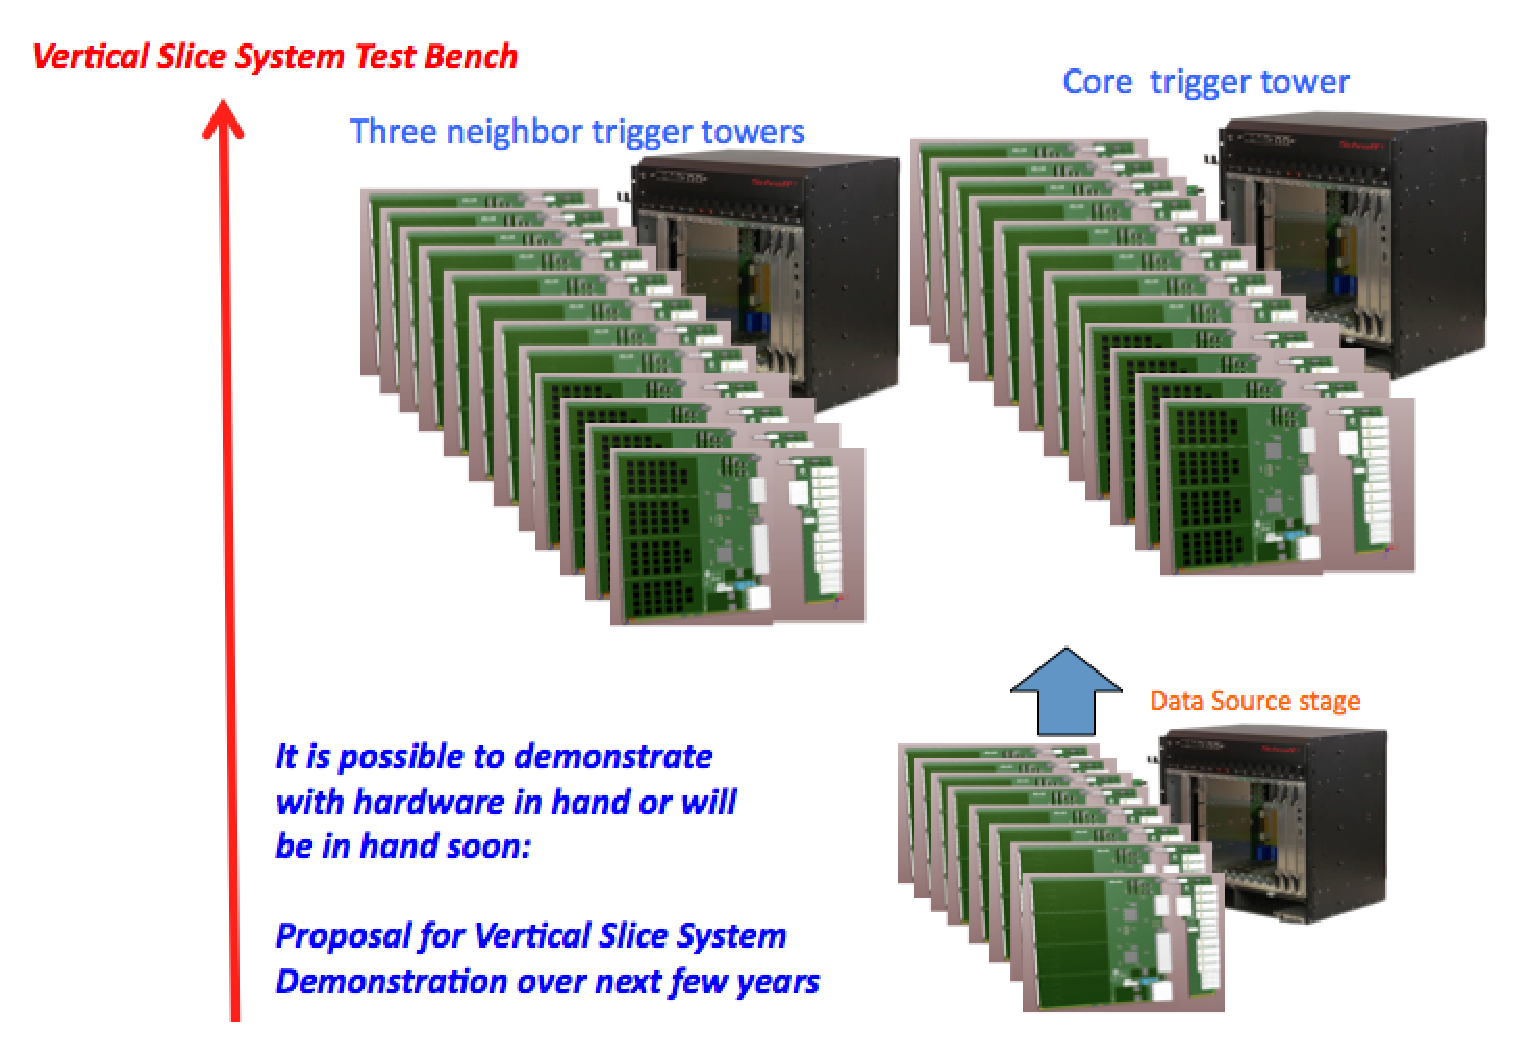
\includegraphics[width=0.8\columnwidth]{Plots/VSTBench.eps}
\caption{Vertical slice test bench principle.}
\label{fig:VS_TBench}
\end{figure}

\subsubsection{Data Source Stage}

\noindent The Data Source mimics the data flow out of the upgraded Phase II outer-tracker running at the HL-LHC. It will drive 300+ fibers (one/module) to the trigger tower under study exactly as the data were coming from the real detector at high luminosity and full speed. Each fiber connection will transmit data at 3.25~Gbps payload bandwidth, in the same way as the actual modules in the future real system. The data will be derived from simulation, appropriately formatted, stored into on-board memories, and then played back at full speed.  The Pulsar IIb board can be used for Data Source stage. 

\subsubsection{Data Input}

\noindent The Data Input Blade (DIB) is responsible for receiving data from the upstream detector electronics (or Data Source output) and transferring them to the PRBs. Up to about 40 fiber links will be received by each DIB. These input links may terminate on the RTM or mezzanine cards. Input fiber links are nominally 3.25~Gb/s payload bandwidth. Again, the Pulsar IIb board can be used as DIB. The Data Input Board will perform zero suppression, pack the stubs into a new format and send them to the PRBs. Current estimates indicate that a rate of about 200 stubs per event per trigger tower, which yields a data rate of roughly 256~Gb/s (200 stubs*32~bits/25~ns) entering each trigger tower on average.

\noindent As an example, in the configuration with eight DIBs and four PRBs, each DIB will be receiving an average of about 256/8 = 32 Gb/s of stub data (after zero suppression). Each of the eight DIBs in the shelf sends data to four PRBs in a round-robin, time multiplexed fashion. Since data is sent to four PRBs, these transfers can take place at a quarter of the input rate, or 32/4 = 8~Gb/s assuming 200 stubs per trigger tower per event.

\noindent In Figure~\ref{fig:VS_TBench}, the ATCA shelf devoted to the "core" trigger tower is shown equipped with 8 DIB boards and 4 PRB boards while the shelf devoted to the "neighbor" towers is equipped with 12 PRB boards, 4 PRB boards for each of the three neighbor towers. In general, each tower needs to share data with 8 neighbors but 3 are sufficient in the demonstration system to test all possible data sharing cases (eta, phi and "diagonal"). Simulated data corresponding to three neighbor towers are delivered from PRB boards in the "neighbor" shelves to the corresponding PRB boards in the "core" shelf.

\subsubsection{Pattern Recognition Board}

\noindent Using again the special configuration above (8 DIB + 4 PRB), each PRB will be receiving 64 Gb/s stub data on average. While receiving the data and sending them to the mezzanine cards, each PRB will exchange data with the corresponding PRB, processing the same time slice, in the neighboring tower for data sharing in the overlap regions. In this case, each PRB can use four 40Gb/s links (QSFP) for the connections in the eta and phi directions, and four 10Gb/s links (SFP+) can be used for data sharing in the "diagonal" directions. The PRB FPGA drives data received from the DIBs to the Pattern Recognition Mezzanine (PRM) boards. This can also be done in a 4x time multiplexed fashion. The 4x time multiplexed transfers from the PRB FPGA to the PRM would require a bandwidth of about 16Gb/s this way. Again, the Pulsar IIb board can be used as PRB. 

 
%\begin{figure}[ht!]
%\centering
%\includegraphics[width=0.4\columnwidth]{Plots/VSTBench_2.eps}
%\caption{}
%\label{fig:VS_TBench_2}
%\end{figure}


\subsubsection{Pattern Recognition Mezzanine Card}

\noindent Each PRB supports four Pattern Recognition Mezzanine (PRM) boards. These boards are based on the FMC standard and support high speed LVDS and SERDES connections to the PRB FPGA. In one possible incarnation, each PRM will contain an FPGA, on board memory to act as Data Buffer, and an array of pattern recognition devices. In our example configuration, we need to support 16~Gb/s between the PRB FPGA and the PRM. The FPGA-PRAM (associative memory) channel bandwidth needs will be a fraction of the PRM input bandwidth, because only relevant stubs will be sent to the relevant pattern recognition chip covering the relevant regions of the trigger tower.


%\begin{figure}[ht!]
%\centering
%\includegraphics[width=0.6\columnwidth]{Plots/VSTBench_3.eps}
%\caption{PRM working principle}
%\label{fig:VS_TBench_3}
%\end{figure}

\noindent  
\noindent

All track fitting algorithms can be implemented in FPGA on the PRMs, therefore they can be studied and compared directly using the same vertical slice demonstration setup. Generally speaking,
PRM's using different approaches to track finding and fitting can be tested and compared within the same overall high-level system architecture and data dispatching scheme. The track fitting can occur on the PRM FPGA. The traditional CDF SVT/FTK-style track fitting stage~\cite{bib:Ann-09} can be used to benchmark the performance of this stage. 

%which is briefly described here. For a region of detector sufficiently small, a linear approximation gives helix %parameters close to those of full helical fit. In other words, for a road narrow enough that a helical fit can be %replaced by a simple linear calculation, each of the 5 helix parameters ($p_i$) can be calculated as the %vector product of prestored constants ($a_{ij}$) and the hit coordinates ($x_j$): $p_i = a_{i0} + %\sum_{i=1}^{N} a_{ij}x_{j}$  where N is the number of coordinates on the track, one for each SCT layer and %two for each pixel layer.  Since there are more than 5 coordinates, there are additional linear equations that %correspond to constraint equations, again where the constants are prestored.  There are (N - 5) such %equations. This linear approximation gives near offline resolution for regions considerably wider than a %single road.  A single set of constants will be used for each sector of the detector. The width of the sector at %each silicon layer is the size of a physical detector module.  Per sector, 5( N + 1) constants are needed for %the helix parameters, and (N - 5)( N + 1) constants are needed for the constraint equations.  The total %number of fit constants (FC) per sector is thus N(N + 1).



